\documentclass[11pt,a4paper]{ctexart}
\usepackage{fontspec}
\defaultfontfeatures{Mapping=tex-text}
\usepackage{xunicode}
\usepackage{xltxtra}
%\setmainfont{???}
\usepackage{amsmath}
\usepackage{amsfonts}
\usepackage{amssymb}
\usepackage{graphicx}
\usepackage{amsthm}
\usepackage{array}
\usepackage{float}   %{H}
\usepackage{booktabs}  %\toprule[1.5pt]
\usepackage[titletoc]{appendix}
\usepackage{tcolorbox} %彩色框框
%===================%插入代码需要的控制
\usepackage{listings}
\usepackage{xcolor}
\lstset{
	numbers=left, 
	numberstyle= \tiny, 
	keywordstyle= \color{ blue!70},
	commentstyle= \color{red!50!green!50!blue!50}, 
	frame=shadowbox, % 阴影效果
	rulesepcolor= \color{ red!20!green!20!blue!20} ,
	escapeinside=``, % 英文分号中可写入中文
} 
%===================%
\usepackage[left=2cm,right=2cm,top=2cm,bottom=2cm]{geometry}

\newtheorem{theorem}{定理}
\newtheorem{definition}{定义}
\newtheorem*{solution}{解}
\newtheorem{practice}{题}
\newcommand{\Sum}[3][i]{\sum\limits_{#1=#2}^{#3}}
\newcommand{\Int}[2]{\int_{#1}^{#2}}
\newcommand{\Sample}[3][X]{{#1}_{#2},\dotsi ,{#1}_{#3}}
\newcommand{\Samiid}[4][X]{{#1}_{#2},\dotsi ,{#1}_{#3}~iid\backsim {#4}}
\newcommand{\norm}[1]{\left\Vert #1\right\Vert_{\infty}}
\newcommand{\diff}[3]{\frac{\partial^{#3}{#1}}{\partial {#2}^{#3}}}
\newcommand{\abs}[1]{\left| {#1}\right|}
\newcommand{\normdis}[2]{N(#1,{#2}^2)}

\title{定性数据统计分析作业 (1)}
\author{钟瑜 \quad 222018314210044}
\date{\today}
\begin{document}
\maketitle
\pagestyle{plain}%设置页码
	
\begin{figure}[H]
	\centering
	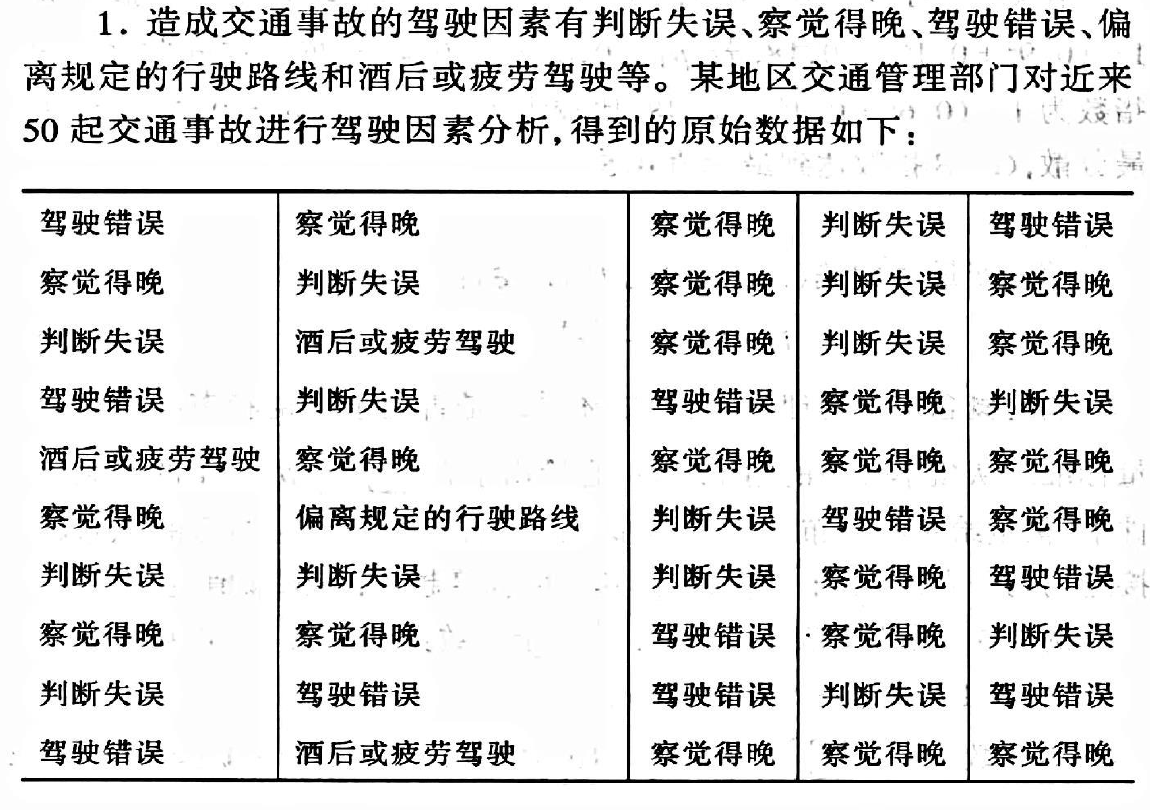
\includegraphics[width=0.7\textwidth]{3.png}
\end{figure}
\begin{figure}[H]
	\centering
	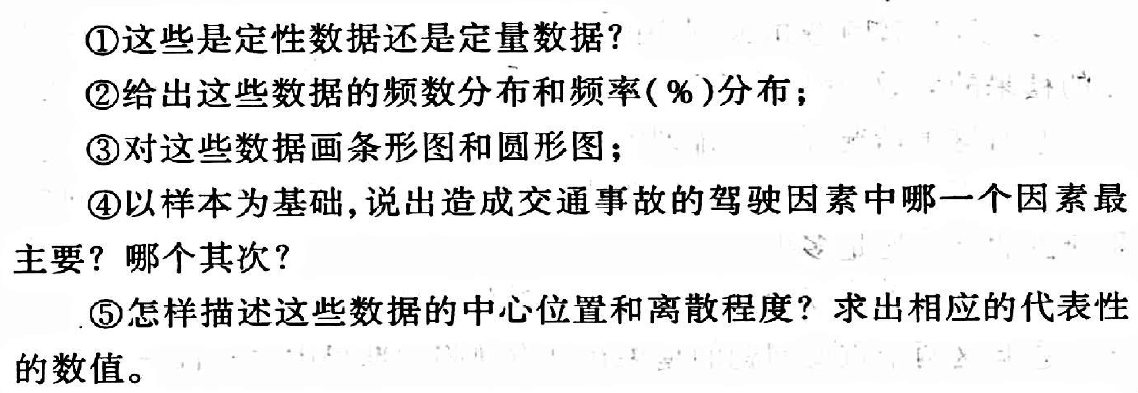
\includegraphics[width=0.7\textwidth]{4.png}
\end{figure}

\begin{solution}
\begin{enumerate}
	\item[1.] 这些数据是定性数据.
	\item[2.] 汇总数据的频数分布和频率分布表如下: 见代码
	\item[3.] 汇总数据的条形图和圆形图:

\begin{figure}[H]
	\centering
	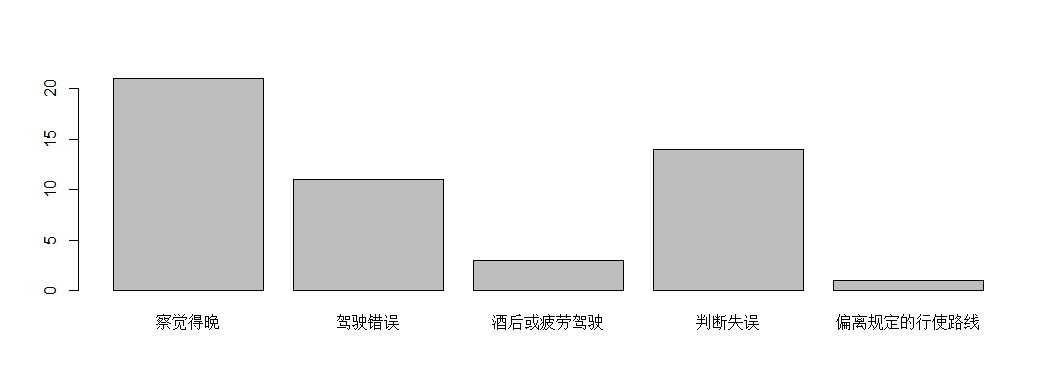
\includegraphics[width=\textwidth]{5.png}
\end{figure}
\begin{figure}[H]
	\centering
	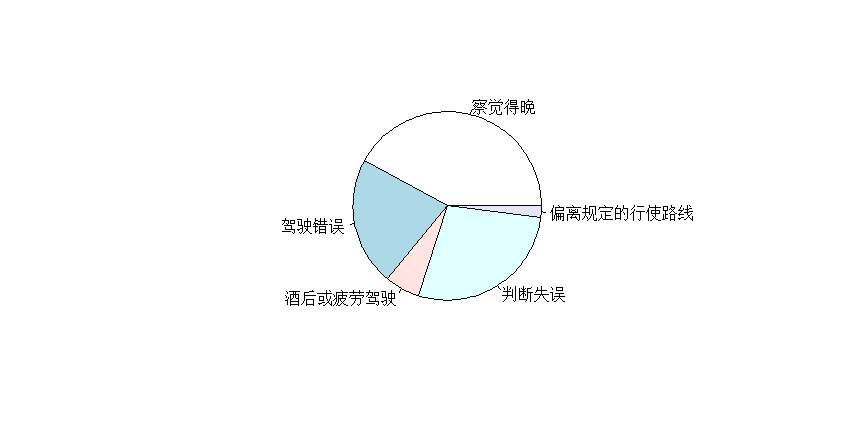
\includegraphics[width=\textwidth]{6.png}
\end{figure}

	\item[5.] 描述数据的中心位置可用众数或者中位数,见代码和下面的帕累托图.
\begin{tcolorbox}[colback=blue!7!white,colframe=blue!40]
	\textbf{帕累托图(Pareto chart)}是将出现的质量问题和质量改进项目按照重要程度依次排列而采用的一种图表。以意大利经济学家V.Pareto的名字而命名的。帕累托图又叫排列图、主次图,是按照发生频率大小顺序绘制的直方图,表示有多少结果是由已确认类型或范畴的原因所造成。
\end{tcolorbox}
\begin{figure}[H]
	\centering
	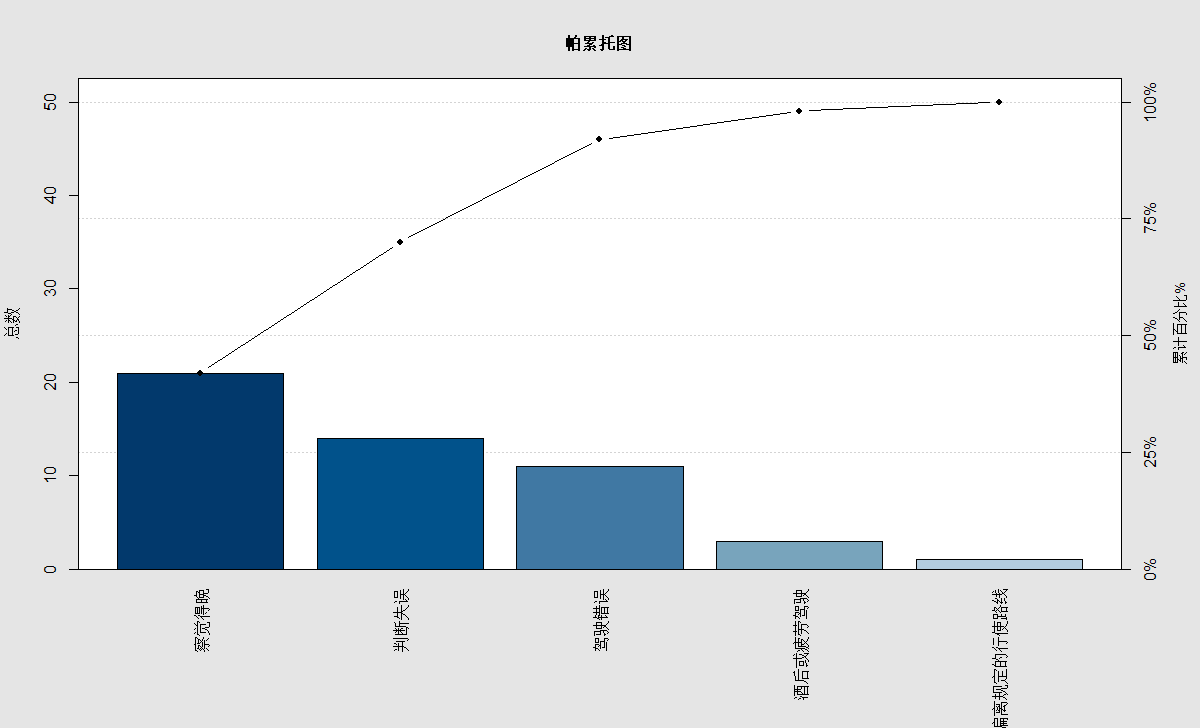
\includegraphics[width=\textwidth]{7.png}
\end{figure}

描述数据的离散程度,见代码.
\end{enumerate}
\end{solution}

\begin{enumerate}
%================================================================%
\item[2.]某学院的学生被要求在完成其课程时填写课程评估调查表.调查表由5类回答尺度的各种问题组成.下列为问题之一,与你已学习的其他课程相比,你现在完成的课程的综合质量怎么样?

$\square$很差   $\square$差    $\square$一般     $\square$好     $\square$很好

某班60个同学在完成了商务统计课程之后给出了下列回答.为了有助于计算机处理调查结果,利用数值尺度1=很差,2=差,3=一般,4=好,5=很好.\\
3 4 4 5 1 5 3 4 5 2 4 5 3 4 4\\
4 5 5 4 1 4 5 4 2 5 4 2 4 4 4\\
5 5 3 4 5 5 2 4 3 4 5 4 3 5 4\\
4 3 5 4 5 4 3 5 3 4 4 3 5 3 3\\
\\
1. 这些是定性数据还是定量数据?\\
2. 给出汇总数据的频数分布和频率分布.\\
3. 给出汇总数据的条形图和圆形图;\\
4. 以你的汇总为基础,解释学生对课程的综合评估.\\
\begin{solution}

\begin{enumerate}
	\item[1.] 这些数据是定性数据.
	\item[2.] 汇总数据的频数分布和频率分布表如下:
\begin{table}[!htbp]   %[H]
	\caption{频数频率分布表}\label{tab:101} \centering
	\begin{tabular}{ccc}
		\toprule[1.5pt]
		等级 & 频数 & 频率\\
		\midrule[1pt]
		 很差& 2 & 0.0333\\
		差 & 4 & 0.0667\\
		一般 & 12 & 0.2000\\
		好 & 24 & 0.4000\\
		很好 & 18 & 0.3000\\
		\bottomrule[1.5pt]
	\end{tabular}
\end{table}
	
	\item[3.] 汇总数据的条形图:
	\begin{figure}[H]
		\centering
		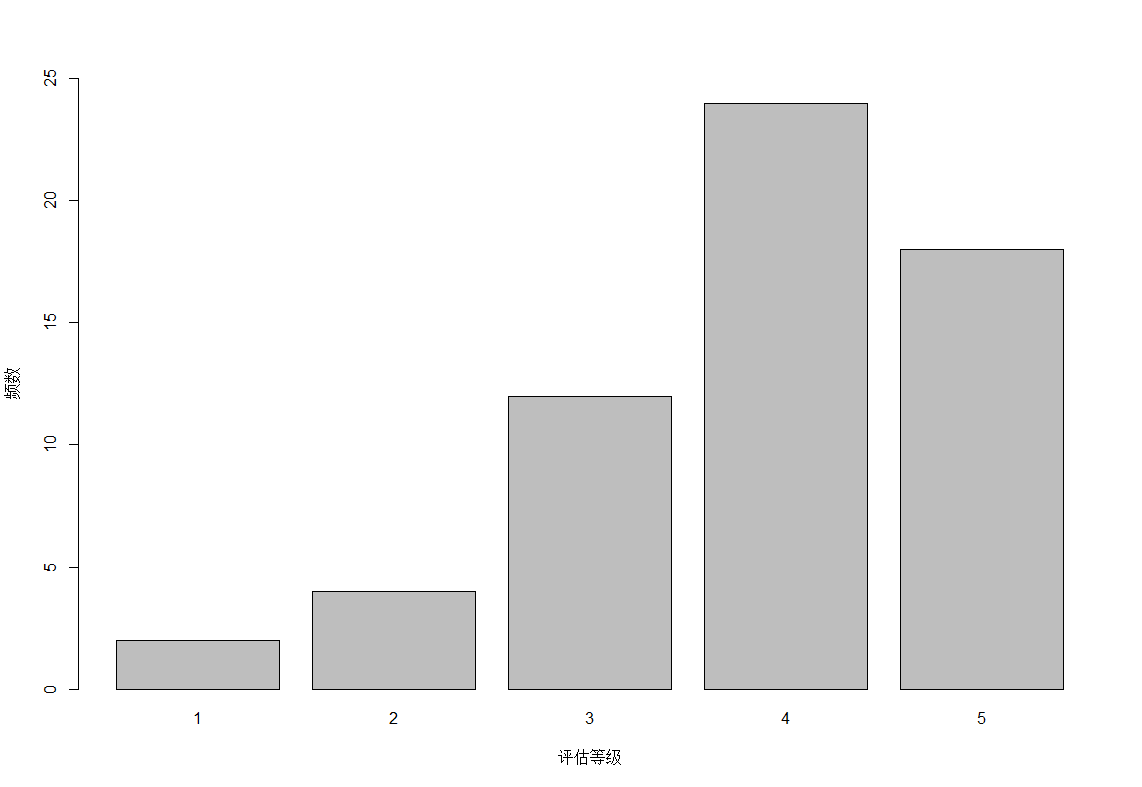
\includegraphics[width=0.7\textwidth]{1.png}
	\end{figure}

给出汇总数据的圆形图:
	\begin{figure}[H]
	\centering
	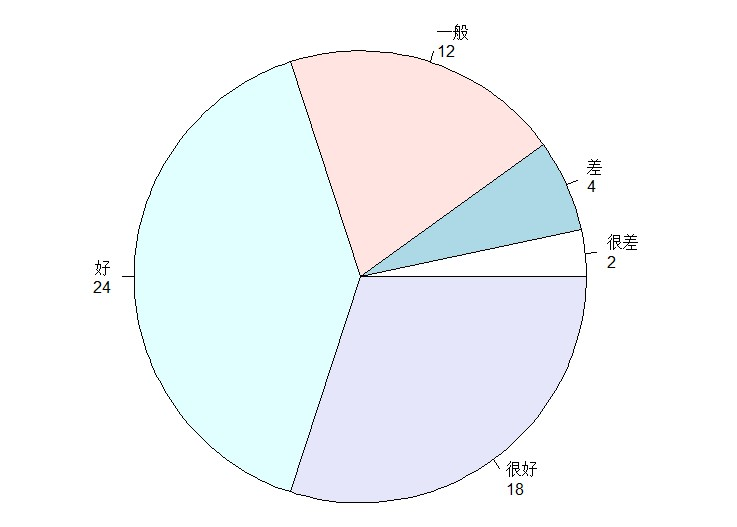
\includegraphics[width=0.7\textwidth]{2.jpg}
	\end{figure}

	\item[4.] 由以上汇总,学生对该课程的综合质量评价主要是好和很好,接近七成;只有十分之一的同学对本课程的综合质量评价为差或很差,因此学生对课程的综合评估总体上看是好的,只有非常少的同学不满意.
\end{enumerate}
\end{solution}
%=================================================================%
\end{enumerate}
\centering\textbf{\Large 附录}
\begin{appendices}

\section{1.2的代码}
\begin{lstlisting}
> a<- read.csv("E:/1.分类数据分析/习题1 频数分布条形图/q1.csv",header = F)
> table(a)             #频数分布
察觉得晚      驾驶错误     酒后或疲劳驾驶 
21            11          3 
判断失误 偏离规定的行使路线 
14       1 
> prop.table(table(a)) #频率分布
察觉得晚           驾驶错误     酒后或疲劳驾驶 
0.42               0.22        0.06 
判断失误 偏离规定的行使路线 
0.28               0.02 
\end{lstlisting}
\section{1.3的代码}
\begin{lstlisting}
> barplot(table(a))    #条形图
> pie(table(a))        #饼图(原型图)
\end{lstlisting}

\section{1.5的代码}
\begin{lstlisting}
> sort(table(a),decreasing = T)          #频数排列
察觉得晚           判断失误           驾驶错误 
21                 14                 11 
酒后或疲劳驾驶 偏离规定的行使路线 
3                  1 

> cumsum(prop.table(table(a)))    #累积百分比
察觉得晚           驾驶错误     酒后或疲劳驾驶 
0.42               0.64               0.70 
判断失误 偏离规定的行使路线 
0.98               1.00 

> library(qcc)
 __ _  ___ ___ 
/ _  |/ __/ __|  Quality Control Charts and 
| (_| | (_| (__   Statistical Process Control
\__  |\___\___|
   |_|           version 2.7
Type 'citation("qcc")' for citing this R package in publications.

> pareto.chart(sort(table(a),decreasing = T),ylab = "总数",
ylab2 = "累计百分比%",main='帕累托图')

Pareto chart analysis for sort(table(a), decreasing = T)
                   Frequency Cum.Freq. Percentage Cum.Percent.
察觉得晚                  21        21         42           42
判断失误                  14        35         28           70
驾驶错误                  11        46         22           92
酒后或疲劳驾驶             3        49          6           98
偏离规定的行使路线         1        50          2          100

> #离散程度的描述
> 1-max(table(a))/sum(table(a))     #离异比率
[1] 0.58
> 1-sum(prop.table(table(a))^2)     #Gini-Simpson指数
[1] 0.6928
> -sum(prop.table(table(a))*log(prop.table(table(a))))     #熵
[1] 1.300934
\end{lstlisting}

\section{2.2的代码}
\begin{lstlisting}[language=r]
> pinggu<-read.csv("E:/分类数据分析/zuoye/1/1.csv",head=FALSE)
> table(pinggu)
pinggu
1  2  3  4  5 
2  4 12 24 18 
> pg.table<-table(pinggu)
> prop.table(pg.table)
pinggu
1          2          3          4          5 
0.03333333 0.06666667 0.20000000 0.40000000 0.30000000 
\end{lstlisting}

\section{2.3的代码}
\begin{lstlisting}[language=r]
> barplot(pg.table,xlab = "评估等级",ylab="频数",ylim=c(0,25))

> lbls<-paste(c("很差","差","一般","好","很好"),"\n",pg.table,sep = "")
> pie(pg.table,labels=lbls)
\end{lstlisting}

\section{绘图笔记}
\begin{tcolorbox}[colback=pink!10!white,colframe=pink!100!black]
\begin{enumerate}
	\item sep 是函数的形式参数,多数情况下, seq 参数用来指定字符的分隔符号。不仅用在你所提到的输出,也用在输入,也用在字符串的合并与拆分上。
	
	csv 文件是用逗号分隔的,故而 sep = "," 
	
	tsv 文件是用制表符分隔的,故而 sep = "\verb|\|t"
	
	常用的分隔符还有空格 sep = " "
	
	分隔符是任意的,可根据具体情况指定的。
	
	\item 函数paste(..., sep = " ", collapse = NULL),字符串使用 paste() 函数来组合。它可以将任意数量的参数组合在一起。以下是所使用的参数的说明:
	
	... - 表示要组合的任何数量的参数。\\
	sep - 表示参数之间的分隔符。它是任选的。\\
	collapse - 用于消除两个字符串之间的空间。但不是在一个字符串的两个词的空间。\\
	\item $ \cdot $ ceiling返回对应数字的'天花板'值,就是不小于该数字的最小整数\\
	$ \cdot $ floor与ceiling相对,返回'地板'值,即不大于该数字的最大值\\
	$ \cdot $ round是R里的'四舍五入'函数,具体的规则采用banker's rounding,即四舍六入五留双规则(wiki)。
	round的原型是round(x, digits = 0), digits设定小数点位置,默认为零即小数点后零位(取整)。
\end{enumerate}
\end{tcolorbox}
\end{appendices}


\end{document}